\chapter{Local Correlation Methods (II): Ground State \label{cha:LOCAL1}}

Since the seminal work of S{\ae}b{\o} and Pulay \cite{Pul1983,Sae1985,Sae1993}, demonstrating how the computational effort of electronic structure methods may be reduced via a local treatment of electron correlation using LMOs and PAOs, the concept of locality has been applied to Hartree-Fock, M{\o}ller-Plesset and Coupled-Cluster methods. Over the years, pure LMO methods have somewhat fallen out of use, in favor for an atomic orbital or (local) natural orbital treatment. This chapter summarizes how the tools and concepts of sparsity and local electron correlation presented in the previous chapter can be used to reduce the scaling of electronic structure methods. The focus will mainly be on Hartree-Fock and M{\o}ller-Plesset, with some words on Coupled-Cluster as well.

\section{Low-Scaling Self-Consistent Field Methods}

Hartree-Fock and density field theory, grouped under the umbrella term of self-consistent field (SCF) methods, are the working horses in quantum chemistry, and the underlying equations, the Roothan and Kohn-Sham equations, are well known and studied. Conventional formulations of HF and DFT, without inclusion of sparsity, scale with $\ccpx{3}$ to $\ccpx{4}$ which hampers extension to very large systems. There are three major bottle-necks: (1) computation of the coulomb matrix, (2) computation of the exchange matrix and (3) diagonalization of the Fock matrix. Over the last couple of decades, multiple different approaches have been proposed on how to lower the scaling of constructing the Fock matrix and circumvent matrix diagonalization. To this day, the field of low scaling SCF methods remains an active area of research in theoretical chemistry. The next sections will address the time-determining steps in detail.

\subsection{The Coulomb Matrix}

Consider again the expression for the coulomb matrix $\mathbf{J}$ 
\begin{equation}
J_{\mu\nu} = \cn{\mu\nu}{\lambda\sigma} P_{\sigma\lambda}
\end{equation}
\noindent which gives the following sparsity diagram:

\begin{center}
\begin{tikzpicture}

\snode{MU}{0,0}{\mu};
\snode{NU}{1,0}{\nu};
\snode{SIG}{2,0}{\sigma};
\snode{LAM}{3,0}{\lambda};

\draw[<->] (MU) -- (NU) node [midway, above] () {S};
\draw[<->] (SIG) -- (LAM) node [midway, above] () {P/S};

\end{tikzpicture}
\end{center}

\noindent The construction of $\mathbf{J}$ has an inherent computational complexity of $\ccpx{2}$, even though the number of non-zero elements scales linearly due to the overlap relationship between $\mu$ and $\nu$. Quadratic scaling algorithms are straight-forward to implement. The first method to construct $\mathbf{J}$ with $\mathcal{O}(N)$ effort was the continuous fast multipole method (CFMM) \cite{Whi1996}. For each element $\mu\nu$ the contributions $\sigma\lambda$ are split into near-field and far-field contributions. NF interactions are computed using standard integration techniques, while FF interactions are computed using multi-level multipole expansion. The linear scaling remains even if the density matrix is not sparse. Other tree-like algorithms were also proposed \cite{Str1996,Cha1996}. In all cases, computing the NF interactions are by far the most time-consuming step.

One way to speed up the evaluation of the non-classical contributions is by moving the contraction step with the density matrix into the underlying integral evaluation. By modifying the formulas for the Gaussian integrals, the explicit storage of the 2-electron repulsion integrals can be skipped which greatly increases computational efficiency \cite{Whi1996,Sha2000,Sha2001}. To this day, the \emph{J engine method}, in combination with CFMM, remains the most efficient way to evaluate the exact Coulomb matrix.

Alternatively, one may introduce the density fitting approximation. The Coulomb matrix is then evaluated in several steps via the intermediates $\mathbf{D}$ and $\mbf{C}$ as 
\begin{align}
J_{\mu\nu} &= C_{X\mu\nu} D_X \\
D_X &= \cn{Y}{\mu\nu} P_{\nu\mu} \\
C_{X\mu\nu} &= \cn{X}{Y}^{-1} \cn{Y}{\mu\nu}
\end{align}
\noindent The computational effort remains unchanged, with $\ccpx{2}$, but with a much lower prefactor, especially for larger, more diffuse basis sets \cite{Wei2002}. Furthermore, the integrals can be recomputed on the fly, and do not need to be explicitly stored. The inversion of the metric matrix $\cn{X}{Y}$ scales cubically, and dominates the cost of the DF approximation for large molecules. 

For large molecules, one could also consider using local density fitting, such as the atomic resolution of the identity or pair-atomic resolution of the identity. Unfortunately, LDF also only reduces the prefactor, rather than scaling. Furthermore, it is necessary to use the robust density fitting of the electron integrals (Equation \ref{eq:DUNLAP}) to recover quadratic scaling in the fitting error, due to the constraints imposed on the density fitting procedure. The Coulomb matrix is then expressed as
\begin{align}
J_{\mu\nu} &= \cn{\mu\nu}{X} b_X + c^Y_{\mu\nu} \left[ g_Y - \tilde{g}_Y \right] \\
g_X &= C^X_{\mu\nu} P_{\mu\nu} \\
\tilde{g}_X &= \cn{X}{Y} b_{Y} \\ 
\quad b_{X} &= C_{\mu\nu}^{X} P_{\mu\nu} 
\end{align}
\noindent The robust LDF-J approximation is evaluated at an effort similar to standard DF-J. The only advantages to LDF in this case pertain to the fitting procedure itself. It is no longer necessary to invert the 2c2e integral matrix $\cn{X}{Y}$, and the fitting coefficients $C_{\mu\nu}^{X}$ can be evaluated in linear scaling fashion. However, it has been demonstrated that using Dunlap's robust formula in combination with local metrics leads to "attractive electron" states where the SCF energy may converge to very high positive values \cite{Mer2013,Hol2014}. The reason is that the the two-electron integral tensor in the robust LDF approximation is no longer positive semidefinite, but \emph{indefinite}, which can lead to severe convergence problems. One way to circumvent this problem is to loosen the constraints on the density fitting procedure, or use a larger auxiliary basis set. In both cases, performance is compromised.  

As shall be shown in chapter \ref{cha:RESULTS}, quasi-robust density offers a better alternative to robust LDF-J methods, with similar sparsity and higher accuracy without the use of Dunlap's formula.

%MEMORY : ON-THE FLY

%POISSON? 
% MANBY, F. R., and KNOWLES, P. J., 2001,Phys.  Rev.Lett.,87,163001.
% MANBY, F. R., KNOWLES, P. J., and LLOYD, A. W., 2001,J. Chem. Phys.,115,9144.

% Str1996 Strain MC, Scuseria GE, Frisch MJ. Achieving linear scaling for the electronic quantum coulomb problem. Science 1996, 271:51–53.
% Cha1996 Challacombe M, Schwegler E, Alml ̈of J. Fast assem-bly of the Coulomb matrix: a quantum chemical treecode.J Chem Phys1996, 104:4685
% Mer2013 Merlot, P.; Kjæ rgaard, T.; Helgaker, T.; Lindh, R.; Aquilante,F.; Reine, S.; Pedersen, T. B.J. Comput. Chem.2013,34, 1486−96.
% Hollman, D. S.; Schaefer, H. F.; Valeev, E. F.J. Chem. Phys.2014,140, 064109.

\subsection{The Exchange Matrix}

\subsubsection{Exact Exchange}

The expression for the exchange matrix is given by 
\begin{equation}
K_{\mu\nu} = \cn{\mu\sigma}{\nu\lambda} P_{\lambda\sigma}
\end{equation}
\noindent In the section where sparsity diagrams were introduced, it was demonstrated that the indices of the exchange expression can be fully linked:
\begin{center}
\begin{tikzpicture}

\snode{MU}{0,0}{\mu};
\snode{NU}{3,0}{\nu};
\snode{SIG}{1,0}{\sigma};
\snode{LAM}{2,0}{\lambda};

\draw[<->] (MU) -- (SIG) node [midway, above] () {S};
\draw[<->] (SIG) -- (LAM) node [midway, above] () {P};
\draw[<->] (LAM) -- (NU) node [midway, above] () {S};

\end{tikzpicture}
\end{center}
\noindent The non-zero elements in $\mathbf{K}$ scale linearly and can be evaluated with $\mathcal{O}(N)$. This property was realized quite early on \cite{Sch1997}. However, a straight-forward implementation where the 4c2e integrals are directly contracted with the density matrix $\mathbf{P}$ using sparse matrix algebra does not give the desired results, when applying the standard $\ccpx{2}$ Schwarz-screening to $\cn{\mu\sigma}{\nu\lambda}$. To lower the scaling of electron integral evaluation, it is important to design a screening algorithm which imposes the P junction between $\sigma$ and $\lambda$ which in turn leads to only a linear increase in the number of bra-ket pairs. 

The ONX method by Schwegler \cite{Sch1997} was the first $\mathcal{O}(N)$ scheme for constructing the exchange matrix, but did not exploit permutational symmetry, which lead to a four fold increase in the prefactor. More competitive methods were proposed later, such as Linear Exchange (LinK) \cite{Och1998}, or symmetrized ONX (SONX) \cite{Sch2000} that could also be applied to small systems without major overhead.

For all approaches, an important step is the screening of the bra-ket pairs using a density-weighted integral estimate
\begin{equation}
|P_{\lambda\sigma}||\cn{\mu\sigma}{\mu\sigma}|^{1/2} |\cn{\nu\lambda}{\nu\lambda}|^{1/2} \leq \tau
\end{equation}
\noindent which scales linearly in the limit of large systems with large HOMO-LUMO gaps. Furthermore, shell ordering is very important to avoid the $\ccpx{2}$ complexity of screening and enable early exit out of the shell loops during construction of the exchange matrix. Similarly to the J kernel, the electron integrals need not to be held in memory, but can be recomputed on the fly.

% https://aip.scitation.org/doi/10.1063/1.472135
% Sch1997 https://aip.scitation.org/doi/10.1063/1.473833
% Och1998 https://aip.scitation.org/doi/10.1063/1.476741
% Sch2000 https://link.springer.com/article/10.1007%2Fs002140000127

\subsubsection{Density Fitting}

The downside of exact linear exchange algorithms is the steep $\ccpx{4}$ scaling with increasing basis set size which delays the onset of the low-scaling regime. For this reason, considerable effort has been invested in recent years to also exploit rank sparsity by density fitting. The DF expression for the exchange matrix in the AO basis reads
\begin{align}
C^X_{\mu\nu} &= \cn{X}{Y}^{-1} \cn{Y}{\mu\nu} \label{eq:DFAOK_STEP1}\\
K_{\mu\nu} &= C^X_{\nu\lambda} \cn{X}{\mu \sigma} P_{\sigma\lambda} \label{eq:DFAOK_STEP2}
\end{align}
\noindent In a straight-forward implementation using sparse matrix algebra, Equation \ref{eq:DFAOK_STEP1} and Equation \ref{eq:DFAOK_STEP2} are evaluated with $\ccpx{3}$  and $\ccpx{2}$ effort respectively. The non-zero elements of both the fitting coefficients $C$ and the 3c2e integrals increase quadratically. Their storage can quickly become problematic for large basis sets if both are held in-core. In principle, both tensors can be recomputed batchwise on-the-fly to reduce memory-footprint, but in contrast to the DF-J kernel where only the 3c2e integrals need to be generated at each iteration, recomputing the fitting coefficients each time introduces a prefactor that is too large for an out-of-core DF-K kernel to be of any practical use (see Chapter \ref{cha:RESULTS}).

For an efficient, direct evaluation of the exchange matrix using density fitting, an MO based approach is much more favorable \cite{Wei2002}. The MO-DF-K kernel is evaluated as
\begin{align}
B^{X}_{\mu i} &= C_{\nu i} \cn{X}{\mu\nu} \\
D^{X}_{\mu i} &= \cn{X}{Y}^{-1/2} B^{X}_{\mu i} \\
K_{\mu\nu} &= B^{X}_{\mu i} B^{X}_{\nu i}
\end{align}
\noindent with cubic computational complexity. The matrix elements of the exchange matrix are evaluated batch-wise over occupied blocks $I$. By contracting the 3c2e integrals with the coefficient matrix $C_{\mu i}$ to form the half-transformed integrals $B^X_{\mu i}$, storage can be reduced from $N_{aux} N_{AO}^2$ to $N_{aux} N_{AO} N_{occ} / N_I$. The 3c2e integrals need to be recomputed for each block $I$, but in practice the number of blocks can be held quite small. The DF-MO-K method is especially well suited for small to medium sized molecules with large diffuse basis sets for post-HF calculations.      

% Wei2002 https://pubs.rsc.org/en/content/articlehtml/2002/cp/b204199p

\subsubsection{Local Density Fitting}

Standard density fitting introduces long-range interactions which inhibit the linear scaling construction of the exchange matrix. This problem can be solved by using LDF. Again, Dunlap's robust density fitting needs to applied to get accurate results. The robust DF-K kernel can take the form
\begin{align}
E_{\mu\nu}^{X} &= C^{X}_{\mu\sigma} P_{\lambda\nu} \\
L_{\mu\nu} &= E_{\mu\sigma}^X \cn{X}{\nu\sigma} - \frac{1}{2} E_{\mu\sigma}^X \cn{X}{Y} C^{Y}_{\nu\sigma} \\
K_{\mu\nu} &= L_{\mu\nu} + L_{\nu\mu}
\end{align}
\noindent All steps can be evaluated in $\mathcal{O}(N)$ time, under the assumption that the fitting coefficients scale linearly:
\begin{center}
\begin{tikzpicture}
\snode{E}{0,0}{E:};
\snode{X}{1,0}{X};
\snode{MU}{2,0}{\mu};
\snode{SIGMA}{3,0}{\sigma};
\snode{NU}{4,0}{\nu};
\draw[<->] (X) -- (MU) node [midway, above] () {LDF};
\draw[<->] (MU) -- (SIGMA) node [midway, above] () {S};
\draw[<->] (SIGMA) -- (NU) node [midway, above] () {P};
\end{tikzpicture}
\end{center}
\begin{center}
\begin{tikzpicture}
\snode{L}{0,0}{L:};
\snode{X}{1,0}{X};
\snode{MU}{2,0}{\mu};
\snode{SIGMA}{3,0}{\sigma};
\snode{NU}{4,0}{\nu};
\snode{PLUS}{5,0}{+};
\snode{X1}{6,0}{X};
\snode{MU1}{7,0}{\mu};
\snode{SIGMA1}{8,0}{\sigma};
\snode{NU1}{9,0}{\nu};
\snode{Y}{10,0}{Y};
\draw[<->] (X) -- (MU) node [midway, above] () {LDF};
\draw[<->] (MU) -- (SIGMA) node [midway, above] () {P};
\draw[<->] (SIGMA) -- (NU) node [midway, above] () {S};
\draw[<->] (X1) -- (MU1) node [midway, above] () {LDF};
\draw[<->] (MU1) -- (SIGMA1) node [midway, above] () {P};
\draw[<->] (SIGMA1) -- (NU1) node [midway, above] () {S};
\draw[<->] (NU1) -- (Y) node [midway, above] () {LDF};
\end{tikzpicture}
\end{center}
\begin{center}
\begin{tikzpicture}

\snode{K}{0,0}{K:};

\snode{MU}{1,0}{\mu};
\snode{NU}{2,0}{\nu};
\snode{PLUS}{3,0}{+};
\snode{MU1}{5,0}{\nu};
\snode{NU1}{4,0}{\mu};

\draw[<->] (MU) -- (NU) node [midway, above] () {};
\draw[<->] (NU1) -- (MU1) node [midway, above] () {};
\end{tikzpicture}
\end{center}

\noindent Alternatively, an LDF-K scheme based on LMOs is also possible \cite{Pol2004,Mej2014}. Over the years, many different LDF-K kernels have been proposed that approximate $C_{\mu\nu}^X$ based on LMO domains \cite{Pol2004,Mej2014}, the atomic resolution of the identity (ARI) \cite{Sod2008}, the pair-atomic resolution of the identity (PARI) \cite{Mer2013} or the concentric atomic density fitting (CADF) \cite{Hol2017}. Although the electron integrals are no longer positive semidefinite, LDF-K is not plagued by the same convergence problems as LDF-J, and it has been shown that LDF-K can be combined with standard DF-J to circumvent convergence problems \cite{Man2015}. 

% Pol2004 https://www.tandfonline.com/doi/abs/10.1080/0026897042000274801
% Sod2007 Hartree-Fock exchange computed using the atomic resolutionof the identity approximation
% Mer2013 https://onlinelibrary.wiley.com/doi/10.1002/jcc.23284
% Mej2014 https://aip.scitation.org/doi/full/10.1063/1.4896199
% Man2015 https://pubs.acs.org/doi/abs/10.1021/ct5008586
% Hol2017 Fast construction of the exchange operator in an atom-centred basis with concentric atomic densityfitting

%\subsubsection{Other Methods}
%
%Other methods for linear-scaling evaluation of Hartree-Fock exchange (also often abbreviated as HFX in literature) are the semi-numerical chain-of-spheres methods (COS) \cite{Nee2009c,Izs2011} and the auxiliary density matrix methods (ADMM) \cite{Gui2010}. For further details, the reader is referred to the original publications. (Maybe elaborate?)

% COS Nee2009 https://www.sciencedirect.com/science/article/pii/S0301010408005089
% COS2 Isz2011 https://aip.scitation.org/doi/full/10.1063/1.3646921
% ADFMM Gui2010 https://pubs.acs.org/doi/10.1021/ct1002225

\subsection{The SCF Procedure}

In the standard SCF procedure, the construction of the Fock matrix is followed by a cubic scaling diagonalization to obtain the MO coefficient matrix and the MO energies. As was discussed in detail in the previous chapter, the eigenvectors of the Fock matrix, i.e. the canonical MOs, are delocalized, and therefore using a sparse eigenvalue solver is unfortunately not an option. The solution is to entirely avoid any MO quantities and replace the Fock diagonalization step. For a functional, fully AO-based method, the same constraints on the density matrix need to be fulfilled as in the standard SCF procedure:
\begin{alignat}{2}
\mathbf{P} &= \mathbf{P}^{\dagger} \qquad &\textrm{Hermiticity}
\\
Tr(\mathbf{PS}) &= N_{ele} \qquad &\textrm{$N$-representability}
\\
\mathbf{PSP} &= \mathbf{P} \qquad &\textrm{Idempotency}
\\
\mathbf{FPS} &- \mathbf{SPF} = \mathbf{0} \qquad &\textrm{Commutator}
\end{alignat}
\noindent There are two main approaches for replacing Fock matrix diagonalization: Purification (or spectral projection) and density matrix minimization \cite{Kim2016}. % (Jor2005).

In spectral projection methods, an initial guess for the density matrix $\mathbf{P}$ of its Fock matrix $\mathbf{F}$ is obtained as
\begin{equation}
\mathbf{P} = \Theta \left( \mu \mathbf{I} - \mathbf{F} \right)
\end{equation}
\noindent where $\mu$ is the chemical potential, and $\Theta$ is the Heaviside step-function. The guess density then has orbital occupation numbers spread between 0 and 1, and has the same eigenvectors as the Fock matrix. The idempotent density is then determined by \emph{density purification}. Density purification is an iterative procedure where a purification transformation is repeatedly applied to the density matrix which converges the orbital occupation numbers either towards 0 or 1. One of the earliest purification transformation by McWeeny \cite{McW1959} takes the form
\begin{equation}
\mathbf{P}_{n+1} = 3\mathbf{P}_n\mathbf{SP}_n - 2\mathbf{P}_n\mathbf{SP}_n\mathbf{SP}_n
\label{eq:MCWEENY}
\end{equation}
\noindent Equation \ref{eq:MCWEENY} is also known as the grand-canonical purification scheme. Other transformations have been proposed over the years, such as canonical purification \cite{Pal1998} or trace-resetting purification \cite{Nik2003}, which do not need the chemical potential $\mu$. The only operations in purification schemes are matrix multiplications, which can be made linearly scaling using sparse matrix algebra. Compared to Fock diagonalization, density purification has a larger overhead, but can be easily integrated without needing large modifications of existing SCF code.

The second method, density matrix minimization, starts from an existing idempotent density matrix guess from a previous SCF cycle and minimizes the energy functional \cite{Li1993,Daw1993,Nun1994}
\begin{equation}
E = Tr\left[ \left(3\mathbf{PSP} - 2\mathbf{PSPSP}\right)\left(\mathbf{K} - \mu \mathbf{I}\right) \right]
\end{equation}
\noindent where $\mathbf{K}$ is the effective one-electron Hamiltonian matrix. The energy minimum is found either by gradient descent or the curvy-step approach \cite{Hel2000,Sha2003}.

Routine application of density matrix purification or minimization has been mainly limited by uncontrolled error accumulation and convergence problems \cite{Rub2008}.

% Jor2005
% McWeeny R. Hartree–Fock theory with nonorthogo-nal basis functions.Phys Rev1959, 114:1528–1529
% Pal1998 A. H. R. Palser and D. E. Manolopoulos, Phys. Rev. B58, 12704~1998!.
% Nik2003 https://aip.scitation.org/doi/pdf/10.1063/1.1559913
% Li1993 https://journals.aps.org/prb/abstract/10.1103/PhysRevB.47.10891
% Daw1993 https://journals.aps.org/prb/abstract/10.1103/PhysRevB.47.10895
% Nun1994 https://journals.aps.org/prb/abstract/10.1103/PhysRevB.50.17611
% Hel2000 https://journals.aps.org/prb/abstract/10.1103/PhysRevB.50.17611
% Sha2003 https://aip.scitation.org/doi/10.1063/1.1558476

\section{M{\o}ller-Plesset}

Second-Order M{\o}ller Plesset is one of the simplest post-Hartree Fock methods available, but still scales as $\ccpx{5}$. Attempts to reduce computational complexity can generally be grouped into two categories: AO-MP2 and LMO-MP2. Independent on which method is used, they share two problems. 

First, the energy denominator in the MP2-amplitudes $t$ make it difficult to transform the MP2 energy expressions into a different basis. AO-MP2 and LMO-MP2 take different approaches to an \emph{orbital-invariant} formulation of the MP2 energy expressions: AO-MP2 solves the problem using the Laplace quadrature, while LMO-MP2 methods generally use the Hylleraas functional. %NO methods can alternatively use canonicalization (Annex \ref{app:CANON}) to use the canonical MP2 expressions. 

Second, steps involving the transformation of the AO two-electron integrals to the Pseudo-AO or LMO basis still remain a major bottle-neck, even with sparsity involved. Both AO- and LMO-MP2 use screening criteria, additional domain restrictions, density fitting or similar methods to lower the cost of integral transformation. These additional procedures are crucial if one wishes to achieve a truly linear scaling MP2 method with a reduced overhead. 

\subsection{Atomic Orbital MP2}

MP2 was first formulated in the AO basis in 1993 by Häser \cite{Has1993}, and a linear scaling algorithm was presented by Scuseria and Ayala in 1999 \cite{Scu1999}. 

\subsubsection{The Laplace Transform}

In 1991, Almlöf showed \cite{Alm1991} that the energy denominator in the MP2 amplitudes can be removed using an integral transform called the \emph{Laplace Transform}

\begin{equation}
\frac{1}{\eps_a + \eps_b - \eps_i - \eps_j} = \int_0^{\infty} e^{-\left(\eps_a + \eps_b - \eps i - \eps_j\right)t} dt
\end{equation}

The t-integration can be replaced \cite{Has1993} by a finite summation using a functional approximation:

\begin{equation}
\frac{1}{\eps_a + \eps_b - \eps_i - \eps_j} \approx \sum_{\alpha}^{n} w\pa e^{-\left(\eps_a + \eps_b - \eps i - \eps_j\right)t\pa}
\end{equation} 

\noindent where $w\pa$ and $t\pa$ are the Laplace weights and exponents at the Laplace points $\alpha$. Accuracy can be controlled by the number of Laplace points $n$. An efficient AO-MP2 implementation heavily relies on an accurate quadrature scheme to achieve the desired accuracy using as few Laplace points as possible to reduce overhead caused by the repeated AO transformation at each step. In general, 5-8 Laplace points are needed to achieve milli-Hartree accuracy, and 10 to 15 points for micro-Hartree accuracy. For more details, the reader is referred to section \ref{sec:LAPLACE}.

\subsubsection{AO-MP2 Equations}

Using the Laplace transform, the energy expression for restricted canonical MP2 can be expressed as
\begin{equation}
\begin{split}
E_{MP2} &= - \sum_{iajb} \frac{\cn{ia}{jb} \left[2 \cn{ia}{jb} - \cn{ib}{ja} \right]}{\eps_a + \eps_b - \eps_i - \eps_j} \\
&\approx - \sum_{\alpha}^n \sum_{iajb} \cn{ia}{jb} \left[2 \cn{ia}{jb} - \cn{ib}{ja} \right] w\pa e^{-\left(\eps_a + \eps_b - \eps i - \eps_j\right)t\pa}
\end{split}
\end{equation}

\noindent The coefficient matrices can then be factored out as
\begin{equation}
\begin{split}
&- \sum_{\alpha}^n \sum_{iajb} \cn{ia}{jb} \left[2 \cn{ia}{jb} - \cn{ib}{ja} \right] w\pa e^{-\left(\eps_a + \eps_b - \eps i - \eps_j\right)t\pa} \\
= &- \sum_{\alpha}^n \sum_{iajb} \sum_{\substack{\mu\nu\lambda\sigma \\ \mu'\nu'\lambda'\sigma'} } w\pa e^{-\left(\eps_a + \eps_b - \eps i - \eps_j\right)t\pa} C_{\mu' i} C_{\sigma' a} \cn{\mu'\sigma'}{\nu'\lambda'} C_{\nu' j} C_{\lambda' b} \\ 
 & \qquad \cross \left\lbrace C_{\mu i} C_{\sigma a} \left [ 2\cn{\mu\sigma}{\nu\lambda} -  \cn{\mu\lambda}{\nu\sigma} \right] C_{\nu j} C_{\lambda b} \right\rbrace  \\
= & - \sum_{\alpha}^n \sum_{\substack{\mu\nu\lambda\sigma \\ \mu'\nu'\lambda'\sigma'}} P\pa_{\mu\mu'} Q\pa_{\sigma\sigma'} \cn{\mu'\sigma'}{\nu'\lambda'} P\pa_{\nu\nu'} Q\pa_{\lambda\lambda'} \left [ 2\cn{\mu\sigma}{\nu\lambda} -  \cn{\mu\lambda}{\nu\sigma} \right] 
\end{split}
\end{equation}

\noindent with the occupied and virtual \emph{pseudo} or \emph{Laplace} density matrices 
\begin{equation}
\begin{split}
P\pa_{\mu\mu'} = \sum_i C_{\mu i} e^{0.25 \ln w\pa + \eps_i t\pa} C_{\mu' i} \\
Q\pa_{\mu\mu'} = \sum_i C_{\sigma a} e^{0.25 \ln w\pa - \eps_a t\pa} C_{\sigma' i}
\end{split}
\end{equation}

\noindent Introducing the \emph{pseudo-AO} transformed electron integrals
\begin{equation}
\cn{\ulgm\olgs}{\ulgn\olgl}\pa = P\pa_{\mu\mu'} Q\pa_{\sigma\sigma'} \cn{\mu'\sigma'}{\nu'\lambda'} P\pa_{\nu\nu'} Q\pa_{\lambda\lambda'}
\label{eq:PSEUDOAOINTS}
\end{equation}

\noindent the energy expression for AO-MP2 then reads
\begin{equation}
E_{AO-MP2} = - \sum_{\alpha}^n \sum_{\mu\nu\lambda\sigma} \cn{\ulgm\olgs}{\ulgn\olgl}\pa \left [ 2\cn{\mu\sigma}{\nu\lambda} -  \cn{\mu\lambda}{\nu\sigma} \right]
\label{eq:AOMP2ENERGY}
\end{equation}

\noindent For $t$ = 0, $\mathbf{P}\pa$ and $\mathbf{Q}\pa$ are equal to the Hartree Fock density matrices. The Laplace matrices also fulfill similar relationships:
\begin{equation}
\mathbf{P}\pa \mathbf{S} \mathbf{P}\pa = \mathbf{0}
\label{eq:PSP0}
\end{equation}
\begin{equation}
\mathbf{P}\pa \mathbf{S} + \mathbf{Q}\pa \mathbf{S} = \mathbf{I}_{exp}
\end{equation}
\noindent where $\mathbf{I}_{exp}$ is a diagonal matrix with trace
\begin{equation}
Tr[\mathbf{I}_{exp}] = \sum_i e^{0.25 \ln w\pa + \eps_i t\pa} + \sum_a e^{0.25 \ln w\pa - \eps_a t\pa}
\end{equation}

\noindent The entries of the pseudo-density also decay exponentially as function of the distance between pseudo-AO centers. Strictly speaking, AO-MP2 is not only formulated in a pure AO-basis ($\mu\nu...$), but also a PAO-like basis ($\ulgm,\olgn,...$). 

\subsubsection{Quadratic Scaling AO-MP2}

Using the linked index rule, the complexity of the AO-MP2 method can easily be determined. The energy expression in Equation \ref{eq:AOMP2ENERGY} involves the dot product between two different tensors, the AO-ERIs $\cn{\mu\sigma}{\nu\lambda}$ and the pseudo-AO-ERIs $\smash{\cn{\ulgm\olgs}{\ulgn\olgl}}\pa$. The scaling is thus determined by the sparsity of those two tensors. From the discussion in Chapter 3, it followed that the ERIs can be computed with $\ccpx{2}$ effort. The pseudo-AO ERIs are computed by transforming the ERIs with the pseudo-density matrices, whose indices $\mu,\nu$ are connected by a P junction. The diagrammatic expression for the pseudo-AO ERIs \ref{eq:PSEUDOAOINTS} is given by
\begin{equation}
\begin{split}
\mu \xlr{P} \mu' \xlr{S} \sigma' \xlr{P} \sigma \\
\nu \xlr{P} \nu' \xlr{S} \lambda' \xlr{P} \lambda
\end{split}
\end{equation}

\noindent Two vertices indicate an $\ccpx{2}$ effort for evaluating Equation \ref{eq:PSEUDOAOINTS}. Therefore, the inherent asymptotic scaling of AO-MP2, without any other further approximations, is $\ccpx{2}$ as well. Similarly to the AO ERIs, a quadratic scaling evaluation of the pseudo-AO ERIs can be achieved using a Schwarz-like screening, as first advocated by Almlöf. Defining the screening matrices

\begin{equation}
\begin{split}
Q_{\mu\nu} &=  \abs{\cn{\mu\nu}{\mu\nu}}^{1/2} \\
X_{\mu\nu} &= \abs{\cn{\ulgm\nu}{\ulgm\nu}}^{1/2} \\
Y_{\mu\nu} &= \abs{\cn{\mu\olgn}{\mu\olgn}}^{1/2} \\
Z_{\mu\nu} &= min\left( \sum_{\sigma} A_{\mu\sigma} \abs{P_{\sigma\nu}}; \sum_{\sigma} B_{\mu \sigma} \abs{Q_{\sigma\nu}} \right)
\end{split}
\end{equation} 

\noindent gives an upper bound for each transformation step in Equation \ref{eq:PSEUDOAOINTS}, for example 

\begin{equation}
\cn{\mu'\sigma'}{\nu'\lambda'} \leq Q_{\mu'\sigma'}Q_{\nu'\lambda'}
\end{equation}
\begin{equation}
\cn{\ulgm\sigma'}{\nu'\lambda'} \leq X_{\mu'\sigma'}Q_{\nu'\lambda'}
\end{equation}
\begin{equation}
\cn{\ulgm \olgs}{\ulgn\olgl} \leq Z_{\mu\sigma} Z_{\nu\lambda}
\end{equation}

\noindent An efficient screening protocol can be devised \cite{Has1993} to get quadratic scaling AO-MP2.

\subsubsection{Linear Scaling AO-MP2}

For the two-electron repulsion integrals, the $1/R$ decay between the charge densities $\cbra{\mu\sigma}$ and $\cket{\nu\lambda}$ is too slow to be of any use even for large systems. However, it was shown \cite{Aya1999} that $bra$ and $ket$ in the Laplace integral tensor $e\pa$ decay much faster with $1/R^3$. Here, we follow the discussion from Reference \cite{Lam2005a}. 

For two non-overlapping charge densities $\cbra{\mu\sigma}$ and $\cket{\nu\lambda}$ the following inequality holds
\begin{equation}
\cn{\mu\sigma}{\nu\lambda} = \cbra{\mu\sigma}\frac{1}{\mathbf{r}_{12}}\cket{\nu\lambda} \leq \frac{1}{R} \left\lvert \sum_{n=0}^{\infty} \frac{\cbra{\mu\sigma} \left( \mathbf{r}_1 - \mathbf{r}_2 \right)^n \cket{\nu\lambda}}{R^n} \right\rvert
\label{eq:MBIESCREEN}
\end{equation}

\noindent Introducing the following abbreviation for the $n$th order 1-center multipole integrals
\begin{equation}
M^{(n)}_{\mu\sigma} = \int \chi_{\mu}(r_1) \mathbf{r}_1^n \chi_{\sigma}(r_1) dr
\end{equation}

\noindent where $M^{0}$ are the overlap integrals, $M^{1}$ are the dipole integrals etc. Rewriting equation \ref{eq:MBIESCREEN} as a multipole expansion gives
\newcommand{\mpole}[2]{M_{#1}^{(#2)}}
\begin{equation}
\begin{split}
\cn{\mu\sigma}{\nu\lambda} &\leq R^{-1} \left\lvert \mpole{\mu\sigma}{0} \mpole{\nu\lambda}{0} \right\rvert + R^{-2} \left\lvert \mpole{\mu\sigma}{1} \mpole{\nu\lambda}{0} - \mpole{\mu\sigma}{0} \mpole{\nu\lambda}{1} \right\rvert \\
&+ R^{-3} \left\lvert \mpole{\mu\sigma}{2} \mpole{\nu\lambda}{0} - 2 \mpole{\mu\sigma}{1} \mpole{\nu\lambda}{1} + \mpole{\mu\sigma}{0} \mpole{\nu\lambda}{2}\right\rvert \\
&+ R^{-4} \left\lvert \mpole{\mu\sigma}{3} \mpole{\nu\lambda}{0} - 3\mpole{\mu\sigma}{2} \mpole{\nu\lambda}{1} + 3\mpole{\mu\sigma}{1} \mpole{\nu\lambda}{2} - \mpole{\mu\sigma}{0} \mpole{\nu\lambda}{3}\right\rvert \\
&+ \mathcal{O}(R^{-5})
\end{split}
\end{equation}

\noindent From equation \ref{eq:PSP0}, it follows that $M_{\ulgm\olgs}^{(0)} = S_{\ulgm\olgs} = 0$. The multipole expansion for the pseudo-AO ERIs $e\pa$ therefore reduces to
\begin{equation}
\begin{split}
\cn{\ulgm\olgs}{\ulgn\olgl} &\leq R^{-3} \left\lvert - 2 \mpole{\ulgm\olgs}{1} \mpole{\ulgn\olgl}{1} \right\rvert \\
&+ R^{-4} \left\lvert - 3\mpole{\ulgm\olgs}{2} \mpole{\ulgn\olgl}{1} + 3\mpole{\ulgm\olgs}{1} \mpole{\ulgn\olgl}{2} \right\rvert \\
&+ \mathcal{O}(R^{-5})
\end{split}
\end{equation}

\noindent which shows the $1/R^3$ dependence of the tensor $\cn{\ulgm\olgs}{\ulgn\olgl}$. Combined with the $1/R$ decay of the AO ERIs, this leads to an overall $1/R^4$ behavior for the AO-MP2 energy. This long-range decay can be exploited to introduce a sparsity relationship between the bra and ket quantities, and reduce the scaling of AO-MP2 from $\ccpx{2}$ to $\ccpx{1}$. In the original paper by Ayala and Scuseria \cite{Aya1999}, this decay was accounted for by introducing an interaction domain centered on each atomic orbital $\mu$ in the form of a sphere. For the integrals $\cn{\ulgm\olgm}{\ulgn\olgn}$, the domain $\mathcal{D}(\mu)$, comprises all charge distributions $\sigma\lambda$ for which 
\begin{equation}
\left( P\pa_{\mu\sigma} S_{\sigma\lambda} Q\pa_{\lambda\mu} \right) \geq \epsilon 
\end{equation}
\noindent The radius $R_{\mu}$ of the interaction sphere is defined by the maximum distance between $\mu$ and the charge density $\sigma\lambda$ in its domain. One can then screen long-range behavior for the interaction sphere $\mu$ and $\nu$ by the distance criterion
\begin{equation}
r_{\mu\nu} - R_{\mu} - R_{\nu} \geq r_0
\end{equation}
\noindent The biggest drawback of the scheme above is that the threshold parameters $r_0$ and $\epsilon$ are system-dependent. 
A more rigorous screening method has been proposed by Lambrecht et al. known as multipole based integral estimates (MBIE) \cite{Lam2005,Lam2005a,Dos2008}. MBIEs offer a tight upper bound for the AO and pseudo-AO electron integrals by using the multipole expansion and replacing the higher order terms $\mathcal{O}(R^{-5})$ by lower-order ones. 

% Pul1983 P. Pulay,Chem. Phys. Lett., 1983,100, 151.27 S. 
% Sae1985 Saebø and P. Pulay,Chem. Phys. Lett., 1985,113, 13
% Alm1991 J. Almlo ̈f, Chem. Phys. Lett.181, 319~1991!
% Has1992 https://aip.scitation.org/doi/abs/10.1063/1.462485
% Has1993 https://link.springer.com/article/10.1007%2FBF01113535
% Aya1999 https://aip.scitation.org/doi/pdf/10.1063/1.478256
% First MBIE Paper: Lam2005 https://aip.scitation.org/doi/pdf/10.1063/1.2079967
% Second MBIE Paper: Lam2005a https://aip.scitation.org/doi/pdf/10.1063/1.2079987
% Improved MBIE Paper: Lam2008 https://pubs.rsc.org/en/content/articlepdf/2008/cp/b804110e

\subsubsection{Cholesky Decomposition of Pseudo-Densities}

As with any method formulated entirely in an AO basis, AO-MP2 suffers from $\ccpx{4}$ scaling with increasing basis set size $N$. The cost associated with larger basis sets can be mitigated by Cholesky decomposition of the pseudo-density matrices (CDD) \cite{Zie2009}. Similar to the orbital localization technique described in Chapter 3, where the (incomplete) CD of the occupied and virtual Hartree-Fock density matrices yields a set of occupied and virtual Cholesky molecular orbitals, the CD of the pseudo-density matrices $\mbf{P}\pa$ and $\mbf{Q}\pa$ yields a set of Cholesky pseudo-molecular orbitals: 
\begin{equation}
\mathbf{P}\pa = \mathbf{\unl{L}}\pa \mathbf{\unl{L}}^{(\alpha)T}
\end{equation}
\begin{equation}
\mathbf{Q}\pa = \mathbf{\ovl{L}}\pa \mathbf{\ovl{L}}^{(\alpha)T}
\end{equation} 
\noindent The pseudo-molecular orbitals show a local behavior inherited from the sparsity of the pseudo-density matrices. It has been observed however \cite{Lue2017}, that the pseudo-MOs $L$ are not always very well localized. A more localized set of MOs can be obtained by using the orthogonalized pseudo-density matrices, for example in the case of $\mathbf{\unl{P}}\pa$:
\begin{equation}
\mathbf{P}\pa_{orth} = \mathbf{S}^{1/2} \mathbf{P}\pa \mathbf{S}^{1/2}
\end{equation}
\noindent The pseudo-MO coefficients are then computed as
\begin{equation}
\mbf{\unl{L}}\pa = \mathbf{S}^{-1/2} \mathbf{\unl{L}}\pa_{orth}
\end{equation}
\noindent The square root and inverse square root of the overlap matrix $\mathbf{S}$ are most reliably found by (full) Cholesky decomposition. The number of occupied and virtual pseudo-MOs is given by the rank of the occupied/virtual pseudo-density matrices, which is equal or a little less than the number of occupied/virtual CMOs. 

One can then formulate the CDD-MP2 energy expression as
\begin{equation}
E_{CDD-MP2} = - \sum_{\alpha}^n \sum_{\uli\ola\ulj\olb} \cn{\uli\ola}{\ulj\olb}\pa \left [ 2\cn{\uli\ola}{\ulj\olb}\pa -  \cn{\uli\olb}{\ulj\ola}\pa \right]
\end{equation}
\noindent with the pseudo-MO integrals
\begin{equation}
\cn{\uli\ola}{\ulj\olb}\pa = \unl{L}\pa_{\mu\uli} \ovl{L}\pa_{\sigma\ola} \cn{\mu\sigma}{\nu\lambda} \unl{L}\pa_{\nu\ulj} \ovl{L}\pa_{\lambda\olb}
\end{equation}
\noindent CDD-MP2 therefore reduces the sizes of the tensors from $N^{4}_{AO}$ to $N_{occ}^2N_{vir}^2$, while still being sparse. Similar to AO-MP2, Schwarz screening and interaction domains can be introduced to obtain quadratic and linear scaling CDD-MP2.

% first appearence of CDD-MP2 Zie2009 https://aip.scitation.org/doi/pdf/10.1063/1.3142592
% AO-RPA Lue2017 https://pubs.acs.org/doi/abs/10.1021/acs.jctc.6b01235

\subsubsection{Density Fitting in AO-MP2}

To reduce the prefactor associated with integral transformation, either from AOs to pseudo-AOs, or from AOs to pseudo-MOs, on can furthermore introduce density fitting \cite{Zie2009,Mau2014}. The transformed 3c2e integrals are given at each Laplace point $\alpha$ by
\begin{equation}
\cn{X}{\ulgm\olgn}\pa = \cn{X}{\mu'\nu'} P\pa_{\mu\mu'} Q\pa_{\nu\nu'}  
\end{equation}
\noindent which are evaluated with $\ccpx{2}$ cost. Using local density fitting approximations, this step can be reduced to approximately $\mathcal{O}(N)$ \cite{Gla2020}.

\subsubsection{Spin-Opposite Scaling}

SOS-MP2 is a cost-efficient variant of MP2 with improved  accuracy (Section \ref{sec:SCSMP2}). One of the advantages of SOS-MP2 is that by omitting the same-spin contributions, the energy expressions can be efficiently factored when using the density fitting approximation \cite{Mau2014,Gla2020}: 
\begin{equation}
\begin{split}
E_{AO-DF-SOS-MP2} &= - c_{os} \sum^{nlap}_{\alpha=1} \sum_{\mu\nu\sigma\lambda} \cn{\ulgn\olgs}{X}\pa \cn{X}{Y}^{-1} \cn{Y}{\ulgn\olgl}\pa \\
& \cn{\mu\sigma}{X'} \cn{X'}{Y'} \cn{Y'}{\nu\lambda}
\end{split}
\end{equation}
\noindent Introducing the intermediates
\begin{equation}
Z\pa_{XY} = \cn{X}{\ulgm\olgs}\pa \cn{\mu\sigma}{Y}
\end{equation}
\begin{equation}
\tilde{Z}\pa_{XY} = \cn{X}{R}^{-1} Z\pa_{RX}
\end{equation}
\noindent a compact energy expression can be obtained which reads
\begin{equation}
E_{AO-DF-SOS-MP2} = - c_{os} \sum^{nlap}_{\alpha=1} \sum_{XY} \tilde{Z}\pa_{XY} \tilde{Z}\pa_{YX} 
\end{equation}
\noindent The computation of $\mathbf{Z}\pa$ is the time-determining step. The sparse map of the intermediate is given by 
%\begin{equation}
%\tikzmark{X}X \quad \mu \xlr{P} \tikzmark{MUP}\mu' \xlr{S} \nu' \xlr{P} \nu; \quad Y 
%\end{equation}
%\begin{tikzpicture}[overlay,remember picture]
%\node (b) at ($(X)!0.5!(MUP)$) {};
%\draw let \p{1}=(b) in node (c) at (\x1,-0.5) {c}; 
%\draw[->,black] (X.south) |- (c.south) -| (MUP.south) ;
%\end{tikzpicture}
\begin{center}
\begin{tikzpicture}

\snode{X}{-1,0}{X};

\snode{MUP}{0,0}{\mu'};
\snode{MU}{0,-1}{\mu};

\snode{NUP}{1,0}{\nu'};
\snode{NU}{1,-1}{\nu};

\snode{Y}{2,-1}{Y};

\draw[<->] (MUP) -- (MU) node [midway, left] () {P};
\draw[<->] (NUP) -- (NU) node [midway, right] () {P};
\draw[<->] (MU) -- (NU) node [midway, below] () {S};
\draw[<->] (MUP) -- (NUP) node [midway, above] () {S};

\end{tikzpicture}
\end{center}
\noindent which suggests that AO-DF-SOS-MP2 has an overall asymptotic scaling of $\ccpx{3}$. With local density fitting, the graph can become fully connected
\begin{center}
\begin{tikzpicture}

\snode{X}{-1,0}{X};

\snode{MUP}{0,0}{\mu'};
\snode{MU}{0,-1}{\mu};

\snode{NUP}{1,0}{\nu'};
\snode{NU}{1,-1}{\nu};

\snode{Y}{2,-1}{Y};

\draw[<->] (MUP) -- (MU) node [midway, left] () {P};
\draw[<->] (NUP) -- (NU) node [midway, right] () {P};
\draw[<->] (MU) -- (NU) node [midway, below] () {S};
\draw[<->] (MUP) -- (NUP) node [midway, above] () {S};

\draw[<->] (X.north) |- (-0.5,0.5) node[above] {LDF} -| (MUP.north);
\draw[<->] (X.north) |- (-0.5,0.5) node[above] {} -| (NUP.north);

\draw[<->] (Y.south) |- (1.5,-1.5) node[below] {LDF} -| (MU.south);
\draw[<->] (Y.south) |- (1.5,-1.5) node[below] {} -| (NU.south);

\end{tikzpicture}
\end{center}

\noindent where "LDF" is the sparsity relationship introduced between the auxiliary density $X$ and the product density $\cbra{\mu\nu}$, which is metric-specific. In the case of quasi-robust density fitting, LDF = S, and the intermediates $\mathbf{Z}\pa$ can be constructed with linear effort. For weaker decay behavior, such as the error function coulomb-attenuated metric, the scaling is intermediate between linear and quadratic \cite{Gla2020}. 

%CAN BE APPLIED TO CC2
% Mau2014 https://aip.scitation.org/doi/full/10.1063/1.4881144
% Gla2020 https://pubs.acs.org/doi/abs/10.1021/acs.jctc.0c00600
% QQR screeening:
% S. A. Maurer, D. S. Lambrecht, D. Flaig, and C. Ochsenfeld, J. Chem. Phys. 136, 144107 (2012). https://doi.org/10.1063/1.3693908
%  S. A. Maurer, D. S. Lambrecht, J. Kussmann, and C. Ochsenfeld, J. Chem. Phys. 138, 014101 (2013). https://doi.org/10.1063/1.4770502

\subsection{Local Molecular Orbital MP2}

While linear scaling MP2 was first achieved using an atomic orbital formulation, the first low-scaling MP2 implementations were actually formulated in a local molecular orbital basis with domain-specific virtual orbitals \cite{Pul1983,Sae1985,Pul1986,Sae1987,Sae1988}. While pure LMO methods are not used very often nowadays, the concepts and tools they introduced are still found in the context of (pair) natural orbitals \cite{Pin2018}.
% Pul1983 https://www.sciencedirect.com/science/article/pii/0009261483807039?via%3Dihub
% Sae1985 https://www.sciencedirect.com/science/article/pii/000926148585003X
% Pul1986 https://link.springer.com/article/10.1007/BF00526697 (ORBITAL INVARIANT)
% Sae1987 https://aip.scitation.org/doi/abs/10.1063/1.452293
% Sae1988 https://aip.scitation.org/doi/abs/10.1063/1.454111
\subsubsection{Laplace Transform MP2}

In the local molecular orbital basis, the Fock matrix is no longer diagonal, and the amplitudes $t_{iajb}$ cannot be easily expressed in a local basis, due to the energy denominator. AO-MP2 tackles this problem by virtue of the Laplace transform. Similarly, one can obtain an energy expression in the LMO basis. The Laplace decomposed MP2 energy is given by
\begin{equation}
E_{MP2} = \sum_{\alpha}^{n} \sum_{iajb} |w\pa| e^{(\eps_i + \eps_j - \eps_a - \eps_j)t\pa} \left[2\cn{ia}{jb} - \cn{ib}{ja}\right] \cn{ia}{jb}  
\label{eq:MP2LAP}
\end{equation}
\noindent Introducing the unitary occupied and virtual LMO-MO transformation matrix $\mathbf{U}$ 
\begin{align}
\ket{i} &= U_{i\uli} \ket{\uli}
\\
\ket{a} &= U_{a\ola} \ket{\ola}
\end{align}
\noindent which is factorized out, Equation \ref{eq:MP2LAP} becomes
\begin{equation}
\begin{split}
E_{MP2} &= \sum_{\alpha}^{n} \sum_{iajb} \sum_{\uli\ola\olb} \sum_{\ulk\olc\ull\old} |w\pa| e^{(\eps_i + \eps_j - \eps_a - \eps_j)t\pa} U_{i\uli} U_{a\ola} \left[2\cn{\uli\ola}{\ulj\olb} - \cn{\uli\olb}{\ulj\ola}\right] U_{j\ulj} U_{b\olb} \\
& \qquad \qquad U_{i\ulk} U_{a\olc} \cn{\ulk\olc}{\ull\old} U_{j\ull} U_{b\old} \\  
&= \sum_{\alpha}^{n} \sum_{\uli\ola\olb} \left[2\cn{\uli\ola}{\ulj\olb} - \cn{\uli\olb}{\ulj\ola}\right] \sum_{\ulk\olc\ull\old} X_{\uli\ulk}\pa Y_{\ola\olc}\pa \cn{\ulk\olc}{\ull\old} X_{\ulj\ull}\pa Y_{\olb\old}\pa \\
&= \sum_{\uli\ola\olb} \left[2\cn{\uli\ola}{\ulj\olb} - \cn{\uli\olb}{\ulj\ola}\right] \mathcal{T}_{\uli\ola\ulj\olb}
\end{split}
\label{MP2LOCEN}
\end{equation}
\noindent with the Laplace amplitudes $\mathcal{T}$ and the Laplace matrices
\begin{equation}
X_{\uli\ulk}\pa = \sum_i U_{i\uli} |w\pa|^{1/4} e^{\eps_i t\pa} U_{k\ulk}
\end{equation}
\begin{equation}
Y_{\ola\olc}\pa = \sum_a U_{a\ola} |w\pa|^{1/4} e^{-\eps_a t\pa} U_{c\olc}
\end{equation}
\noindent Equation \ref{MP2LOCEN} is the general expression for the MP2 energy in a local molecular orbital basis, where both the occupied and virtual orbitals are \emph{orthogonal}. The situation changes slightly when using non-orthogonal, domain-specific PAOs $\olgm$, which are related to CMOs via
\begin{align}
\ket{\olgm} &= \bar{C}_{\mu a} \ket{a} \\
\ket{a} &= \bar{C}_{\nu a} S_{\olgn\olgm}^{-1} \ket{\olgm} 
\end{align}
\noindent with $\mathbf{S}$ being the overlap matrix in the PAO basis, and $\mbf{\bar{C}} = \mbf{SC}$ are the orthogonalized MO coefficients. The inverse of $\mbf{S}$ is computed by canonical orthogonalization (Appendix \ref{app:LINDEP}). This approximate inverse will be given by the matrix $\mbf{V}$, which is also specific to a given pair $[ij]$. In general, only the virtual CMOs are transformed to the PAO base. The virtual Laplace matrix then takes the following form \cite{Kat2008}:
\begin{equation}
\mathbf{Y}\pa = \mathbf{V} \mathbf{B}\pa \mathbf{V} \pdg 
\end{equation}
\begin{equation}
B_{\olgm\olgn}\pa = \sum_a \bar{C}_{\mu a} |w\pa|^{1/4} e^{-\eps_a t\pa} \bar{C}_{\nu a}
\end{equation}
\noindent with the other expressions of the LMO-MP2 energy remaining the same as before.

% Kat2008 https://pubs.rsc.org/en/content/articlepdf/2008/cp/b802993h

\subsubsection{Hylleraas Functional}

Alternatively, the local MP2 amplitudes can be determined iteratively via an orbital-invariant formulation of the MP2 energy expression based on the \emph{Hylleraas functional} \cite{Hyl1929,Pul1986}. The  Hylleraas functional form of the energy is given by minimizing 
\begin{equation}
E^{(2)} = min \left[ 2\bra{\Psi^{(1)}} \mathbf{H} - E_0  \ket{\Psi^{(0}} - \bra{\Psi^{(1)}} \mathbf{H}_0 - E_0 \ket{\Psi^{(1)}} \right]
\label{eq:HYLMIN}
\end{equation}
\noindent In the case of MP2, the quantities in Equation \ref{eq:HYLMIN} take the form
\begin{equation}
\bra{\Psi^{(1)}} \mathbf{H} - E_0  \ket{\Psi^{(0)}} = \frac{1}{4} \sum_{ijab} t_{iajb} \sbra{ij}\sket{ab}
\end{equation}
\begin{equation}
\bra{\Psi^{(1)}} \mathbf{H}_0 - E_0 \ket{\Psi^{(1)}} = \frac{1}{8} \sum_{ijabc} t_{iajb} f_{cb} t_{iajc} - \frac{1}{8} \sum_{ijkab} t_{iajb} f_{jk} t_{iakb}
\end{equation}
\noindent Minimization of the MP2 Hylleraas functional, with respect to the amplitudes $\mathbf{t}$ yields a set of linear equations given by
\begin{equation}
\begin{split}
R_{iajb} = \bra{ij} {} \ket{ab} + \sum_c \left(t_{ijab} f_{cb} + f_{ac} t_{iacb} \right) - \sum_k \left( t_{iakb} f_{kj} + f_{ik} t_{kajb} \right) = 0
\end{split}
\label{eq:MP2RES}
\end{equation}
\noindent where $\mathbf{R}$ is the residual. The amplitudes $\mathbf{t}$ are then no longer computed directly by a closed expression, but iteratively by solving the system of equations, in a similar vein to coupled cluster. %This method is said to be orbital invariant, because any molecular orbital representation can be used. 
For a set of orthogonal MOs $\uli$ and $\ola$, the quantities in Equation \ref{eq:MP2RES} are simply replaced by their local equivalent. Analogous to LT-LMP2, if PAOs are to be used for the virtual orbital space, the non-orthogonality needs to be taken into consideration. For a mixed LMO-PAO basis, the MP2 residual reads
\begin{equation}
\begin{split}
R_{\uli \olgm \ulj \olgn} = & \bra{\uli\ulj}{}\ket{\olgm\olgn} + \sum_{\olgs\olgl} \left( f_{\olgm\olgs} t_{\uli \olgs \ulj \olgl} S_{\olgl\olgn} + S_{\olgm\olgs} t_{\uli \olgs \ulj \olgl} f_{\olgl\olgn} \right) \\
&-  \sum_{\ulk} \left( f_{\uli \ulk} S_{\olgm\olgs} t_{\ulk \olgs \ulj \olgl} S_{\olgl \olgn} + f_{\ulk \ulj} S_{\ulgm\olgs} t_{\uli \olgs \ulj \olgl} S_{\olgl\olgn} \right) = 0
\end{split} 
\end{equation}
\noindent For specific virtual orbitals, the equations are solved individually for each electron pair $ij$ to obtain their amplitude $\mathbf{t}_{ij}$ and to compute the pair correlation energy. 

\subsubsection{Quadratic Scaling LMP2}

Similar to CEPA, the MP2 energy can be computed as a sum of electron pair energies
\begin{equation}
E_{MP2} = \sum_{ij} e_{ij}
\end{equation}
\begin{equation}
e_{ij} = \left( 2t_{ij}^{ab} - t_{ij}^{ba} \right) \cn{ia}{jb} 
\end{equation} 
 \noindent For well localized orbitals, the electron pair correlation $e_{ij}$ decays with $1/r_{ij}^6$ with the distance between orbital centers. Electron pairs are generally divided into four groups: strong pairs ($r_{ij} < 1a_0$), weak pairs ($1a_0 < r_{ij} \leq 8 a_0$), distant pairs ($8 < r_{ij} \leq 15 a_0$), and very distant pairs ($15 < r_{ij}$) \cite{Sch1999}. Other than by distance criteria, electron pairs can be grouped by their pair energy \cite{Nee2009}. Figure \ref{fig:EPAIRS} shows the number of significant electron pairs in each category for glycine chains. The number of strong, weak and distant pairs scale as $\mathcal{O}(N)$, while the number of very distant pairs scales quadratically. 

The occupied molecular orbitals $ij$ are localized using e.g. Foster-Boys, Pipek-Mezey or a Cholesky decomposition of the density matrix. Virtual orbitals are generally localized by projection onto the atomic orbital space (PAOs) and subsequently assigning them to pair domains $[ij]$ (domain specific virtuals), or by diagonalizing the MP2 density matrix for each electron pair (pair natural orbitals).  In all cases, the number of virtual orbitals within a domain scales as $\mathcal{O}(1)$ for each electron pair $ij$, in the limit of large molecules, such that the scaling of LMP2 is determined by the scaling of significant electron pairs only.

The major bottle-neck in LMP2 is, as usual, the transformation of the 2 electron integrals from the AO basis into the local basis
\begin{equation}
\cn{\uli\ola}{\ulj\olb} = L_{\mu \uli} L_{\sigma \ola} \cn{\mu\sigma}{\nu\lambda} L_{\nu \ulj} L_{\lambda \olb}
\end{equation}
\noindent The expression above translates into the sparsity diagram
\begin{center}
\begin{tikzpicture}

\snode{MU}{0,0}{\mu};
\snode{SIG}{1,0}{\sigma};
\snode{NU}{2,0}{\nu};
\snode{LAM}{3,0}{\lambda};

\snode{I}{0,-1}{\uli};
\snode{A}{1,-1}{\ola};
\snode{J}{2,-1}{\ulj};
\snode{B}{3,-1}{\olb};

\draw[<->] (MU) -- (SIG) node [midway, above] () {S};
\draw[<->] (NU) -- (LAM) node [midway, above] () {S};
\draw[<->] (I) -- (MU) node [midway, below] () {};
\draw[<->] (A) -- (SIG) node [midway, below] () {};
\draw[<->] (J) -- (NU) node [midway, below] () {};
\draw[<->] (B) -- (LAM) node [midway, below] () {};
\draw[<->] (I) -- (A) node [midway, below] () {};
\draw[<->] (J) -- (B) node [midway, below] () {};

\end{tikzpicture}
\end{center}
\noindent which indicates that the MO integrals can be evaluated with $\ccpx{2}$ effort without further approximations. One thing to note is that the quadratic scaling is also obtained, even if the sparsity relationships $i \leftrightarrow a$ and $j \leftrightarrow b$ did not exist, i.e. where virtual orbitals are localized, but not grouped into (pair) domains. The major disadvantage of such non-pair specific methods is that the virtual orbital space is less compact, which leads to a high overhead for integral transformation involving virtual orbitals, which could be the reason that there are no examples in literature using such a scheme. Establishing an a priori sparsity relationship between occupied and virtual space allows to more easily reach the low-scaling regime. 

\begin{figure}
\centering
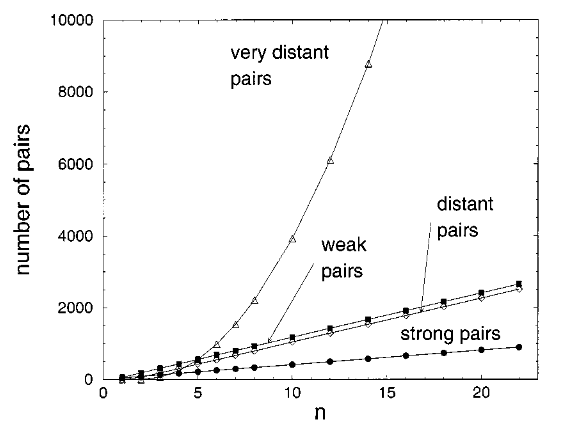
\includegraphics[scale=0.5]{Pics/electron_pairs.png}
\caption[Number of significant electron pairs in glycine chains.]{Number of significant electron pairs in glycine chains. Taken from \cite{Sch1999}}
\label{fig:EPAIRS}
\end{figure}

\subsubsection{Linear Scaling LMP2}

It has been found \cite{Sae1987} early on that the quadratic scaling very distant electron pairs can be safely ignored without major impact on the total correlation energy. Distant pairs may also be approximated either by a multipole expansion \cite{Het1998} or empirically \cite{Rau1995}. As a consequence, this establishes a sparsity relationship between $i$ and $j$, and the sparsity diagram for the MO integrals becomes fully connected
\begin{center}
\begin{tikzpicture}

\snode{MU}{0,0}{\mu};
\snode{SIG}{1,0}{\sigma};
\snode{NU}{2,0}{\nu};
\snode{LAM}{3,0}{\lambda};

\snode{I}{0,-1}{\uli};
\snode{A}{1,-1}{\ola};
\snode{J}{2,-1}{\ulj};
\snode{B}{3,-1}{\olb};

\draw[<->] (MU) -- (SIG) node [midway, above] () {S};
\draw[<->] (NU) -- (LAM) node [midway, above] () {S};
\draw[<->] (I) -- (MU) node [midway, below] () {};
\draw[<->] (A) -- (SIG) node [midway, below] () {};
\draw[<->] (J) -- (NU) node [midway, below] () {};
\draw[<->] (B) -- (LAM) node [midway, below] () {};
\draw[<->] (I) -- (A) node [midway, below] () {};
\draw[<->] (J) -- (B) node [midway, below] () {};
\draw[<->] (I) |- (1,-2.0) node [below] {$1/R^6$} -| (J);

\end{tikzpicture}
\end{center}
\noindent Linear scaling MP2 can therefore be achieved with an LMO formulation \cite{Sch1999}.

% Sch1999 https://aip.scitation.org/doi/pdf/10.1063/1.479957
% distant pairs multipole approximate very distant pairs by multipole expansion Het1998 https://www.sciencedirect.com/science/article/pii/S0009261498004916
% distant pairs Empirically Rau1995 G. Rauhut, J. W. Boughton, and P. Pulay, J. Chem. Phys., 103, 5662 1995 .
%Instead of using distance criteria, can use screening: 
%https://aip.scitation.org/doi/10.1063/1.4773581
\subsubsection{Density Fitting for LMP2}

While specific virtual orbitals form a very compact representation of the virtual space, the fact that each electron pair has their own orthogonal virtual orbital basis means that the total number of virtuals can become exceedingly large, and consequently increases the cost associated with the AO-MO transformation step. The most expensive step then becomes
\begin{equation}
\cn{\uli\ola}{P} = L_{\mu\uli} \cn{\mu\nu}{P} L_{\nu\ola}
\end{equation}
\noindent Transformation of the 3c2e integrals scales with $\ccpx{2}$. Linear scaling can be achieved by introducing an orbital-specific fitting domain $[i]_{fit}$, e.g. by assigning all auxiliary functions $P$ on atoms with a Mulliken charge above a given threshold for the local orbital $i$ \cite{Pin2015}, or by using a Boughton-Pulay like scheme \cite{Wer2015}. This yields the sparsity diagram
\begin{center}
\begin{tikzpicture}

\snode{P}{-1,0}{P};
\snode{MU}{0,0}{\mu};
\snode{SIG}{1,0}{\sigma};

\snode{I}{0,-1}{\uli};
\snode{A}{1,-1}{\ola};

\draw[<->] (MU) -- (SIG) node [midway, above] () {S};
\draw[<->] (I) -- (MU) node [midway, below] () {};
\draw[<->] (A) -- (SIG) node [midway, below] () {};
\draw[<->] (I) -- (A) node [midway, below] () {};
\draw[<->] (I) -- (-1,-1) node [below] {LDF} -- (P);

\end{tikzpicture}
\end{center}
\noindent As opposed to SOS-AO-MP2, where density fitting can give a more favorable factorization of the energy expression, the MO integrals need to be fully assembled for LMP2 in order to solve the linear equations \ref{eq:MP2RES}. The assembly is done in two steps
\begin{align}
B^{X}_{\uli\ola} &= \sum_{Y \in [i]_{fit} \cup [j]_{fit}} \cn{X}{Y}^{-1/2} \cn{Y}{\uli\ola}
\\
\cn{\uli\ola}{\ulj\olb} &= \sum_{X \in [i]_{fit} \cup [j]_{fit}} B^{X}_{\uli\ola} B^{X}_{\ulj\olb} 
\end{align}
\noindent The two steps are repeated for each electron pair $ij$, and the sum runs over all auxiliary functions $P$ in the unified fitting domain $[i]_{fit} \cup [j]_{fit}$, which enforces linear scaling for these steps as well. 

% Pin2015 https://aip.scitation.org/doi/pdf/10.1063/1.4926879
% Wer2015 https://pubs.acs.org/doi/pdf/10.1021/ct500725e

\subsection{Natural Orbitals}

Pure natural orbital techniques are generally not used in the context of MP2, given that MP2 is also used as a guess density to obtain the natural orbitals. Rather, NOs are more popular in the context of coupled cluster methods like CCSD and CCSD(T), though there have been some application in the context of PNOs \cite{Fra2017,Sch2013} and domain-based local PNOs (DLPNO) \cite{Wer2015,Pin2018}. The latter combines the compact virtual representation of PNOs with the local electron-pair treatment of LMOs   described in the previous sections. 

As was previously explained, the main idea of NOs is to truncate the virtual space by omitting all orbitals with an occupation number below a certain threshold. The MO integrals in the truncated NO basis can then be plugged into one of the orbital-invariant formulations of the MP2 energy expressions, or they can be canonicalized to be used in the standard MP2 expressions.

\section{Coupled Cluster}

Virtually all of the concepts introduced in the previous section can also be applied in the context of coupled cluster. Local MP2 and local CC evaluate the MO integrals in the same exact manner, either using LMOs \cite{Sch2001, Sch2002, Sch2000a, Sch2000b,Sch2001}, natural orbitals \cite{Tau2008,Nag2018,Rol2013} or pair-natural orbitals \cite{Nee2009a,Guo2018,Sch2017,Rip2013}. The orbital-invariant CC amplitude equations can then be directly solved at a reduced cost by plugging in the truncated MO integrals.

An atomic orbital formulation of the coupled cluster equations is possible \cite{Scu1999}, but has never been pursued further. Again, the AO-CCSD method as presented by Scuseria et al. is not really a pure AO-method, but rather a PAO-like approach similar to PAO-CCSD later proposed by Christiansen and Koch \cite{Chr2006}. The reason why AO/PAO coupled cluster methods have not been popular is likely due to the very high prefactor for larger basis sets, which are often crucial for obtaining accurate correlation energies. Moreover, in contrast to MP$n$ amplitudes, the coupled cluster amplitudes do not have closed expressions, which in turn inhibits any further factorizations of coefficient matrices to reduce the overhead like in Cholesky decomposed MP2, with the exception of hybrid methods like CC2 \cite{Sac2021}.

%AO: Scu1999
%LNO: Nag2018 (CCSD(T)) Rol2013 (CCSD(T), 
%PNO: Nee2009, Guo2018 (CCSD(T) DPLNO), LPNO CCSD(T) Sch2017, Rip2013 CCSD, 
%LMO: Sch2001 (CCSD), Sch2002 (CCSDT) Sch2000, Sch2000a (CCSD(T)) , 
%FNO Bar2005

%\subsection{Atomic Orbital CC2}
%
%The atomic orbital approach for low scaling MP2 can be extended to CC2 ... currently under work
%
%\subsection{Atomic Orbital CCSD: PAO or AO?}
%
%!!!!!!!!!!!!! REWRITE !!!!!!!!!!!!!!!!
%As opposed to MP2 and CC2, where the energy denominator in the closed form expression for the doubles amplitudes $t_{iajb}$ makes it difficult to find an orbital-invariant representation of the energy expressions, it is much easier to do so for CCSD. The restricted CCSD correlation energy expression reads
%\begin{equation}
%E_{corr} = \sum_{ijab} v_{iajb} t^{CCSD}_{iajb} \qquad v_{iajb} = 2\cn{ia}{jb} - \cn{ib}{ja} 
%\end{equation}   
%\noindent In their 1999 paper [ref], Scuseria and Ayala have shown that there are two possible "AO" representations of the CCSD correlation energy. The first and most straight-forward approach is to factor out the MO coefficient matrices from the MO electron repulsion integrals $v$, similar to AO-MP2
%\begin{equation}
%\begin{split}
%E_{corr} &= \sum_{ijab} \sum_{\mu\nu\sigma\lambda} C_{\mu i} C_{\sigma  a} v_{\mu\sigma\nu\lambda} C_{\nu j} C_{\lambda b} t_{iajb} \\
%&= \sum_{\mu\nu\sigma\lambda} v_{\mu\sigma\nu\lambda} t_{\ulgm\olgs\ulgn\olgl}
%\end{split} 
%\end{equation}
%\noindent whith the amplitudes $\mathbf{t}$ recast in a PAO-like basis:
%\begin{equation}
%t_{\ulgm\olgs\ulgn\olgl} = C_{\mu i} C_{\sigma a} t_{iajb} C_{\nu j} C_{\lambda b}
%\end{equation}
%\noindent The MO amplitudes can be recovered with
%\begin{equation}
%t_{iajb} = \ovl{C}_{\mu i} \ovl{C}_{\sigma a} t_{\ulgm\olgs\ulgn\olgl} \ovl{C}_{\nu j} \ovl{C}_{\lambda b}
%\end{equation}
%\noindent It should be noted that $\ulgm$, $\olgs$, $\ulgn$ and $\olgl$ do not correspond to the definition of PAOs given in Section .... As opposed to standard PAOs, they lack the overlap matrix $\mathbf{S}$ in the MO-PAO transformation and vice-versa (compare Equation ... with Eqaution ...). Here, the occupied and virtual PAO-like spaces are not mutually orthogonal, but related through the overlap matrix, similar to the pseudo-PAOs used in AO-MP2
%\begin{equation}
%\mathbf{PSQ} = \mathbf{0} \qquad \mbf{P} + \mbf{Q} = \mbf{S}^{-1}
%\end{equation}
%\noindent This alternative PAO-like formulation will be referred to as \emph{mutually non-orthogonal projected atomic orbitals} (or mnoPAOs) from here on out.    
%
%\noindent Instead of using this mnoPAO approach, Scuseria and Ayala proposed an alternative formulation where the coefficient matrices are factored out from the t-amplitudes instead, using the PAO backtransformation \ref{CMO2PAO}:
%\begin{equation}
%\begin{split}
%E_{corr} &= \sum_{ijab} \sum_{\mu\nu\sigma\lambda} v_{iajb} C_{\mu i} C_{\sigma  a} \theta_{\ulgm\olgs\ulgn\olgl} C_{\nu j} C_{\lambda b} \\
%&= \sum_{\mu\nu\sigma\lambda} \Pi_{\ulgm\olgs\ulgn\olgl} \theta_{\ulgm\olgs\ulgn\olgl}
%\end{split} 
%\end{equation}
%\noindent The PAO-amplitudes $\theta$ are related to the MO quantities by
%\begin{equation}
%\theta_{\ulgm\olgs\ulgn\olgl} = \ovl{C}_{\mu i} \ovl{C}_{\sigma a} t_{iajb} \ovl{C}_{\nu j} \ovl{C}_{\lambda b}
%\end{equation}
%\begin{equation}
%t_{iajb} = C_{\mu i} C_{\sigma a} \theta_{\ulgm\olgs\ulgn\olgl} C_{\nu j} C_{\lambda b}
%\end{equation}
%\noindent The mnoPAO and PAO t-amplitudes are related by
%\begin{equation}
%\theta_{\ulgm\olgs\ulgn\olgl} = S_{\mu\mu'} S_{\olgs\olgs'} t_{\ulgm'\olgs'\ulgn'\olgl'} S_{\ulgn\ulgn'} S_{\olgl\olgl'}  
%\end{equation}
%\begin{equation}
%\theta_{\ulgm\olgs\ulgn\olgl} = P_{\mu\mu'} P_{\olgs\olgs'} \theta_{\ulgm\olgs\ulgn\olgl} P_{\ulgn\ulgn'} P_{\olgl\olgl'} 
%\end{equation}
%!!!!! REWRITE !!!!!!!!!!!
%
%\subsection{Local Coupled Cluster}
%
%\subsection{FNO Coupled Cluster ??}
%
%\section{Critical Stance on AO vs LMO} 
%
%Distance criteria, or Mulliken/Löwdin pouplation
%AO only for closed expressions (not for CCSD++) 
%LOcal: ij cirteria, ij->ab criteria % https://www.sciencedirect.com/science/article/pii/S1574140006020044?via%3Dihub
%
%% Hylleraas functional: 
%% Hyl1930 https://link.springer.com/article/10.1007/BF01397032
%
%% First use of LMO+PNOs with Hylleraas 
%% Pul1986 https://link.springer.com/article/10.1007%2FBF00526697
%
%% LInear scaling of the functional
%% Linear scaling of electron inetgrals
%% linear scaling of MO-AO transformation -> or density fitting

%\section{Summary}
%
%LMO vs PNO vs NO ?